% Figure LaTeX snippets. Intended to be copied into main.tex.

\begin{figure}[t]
  \centering
  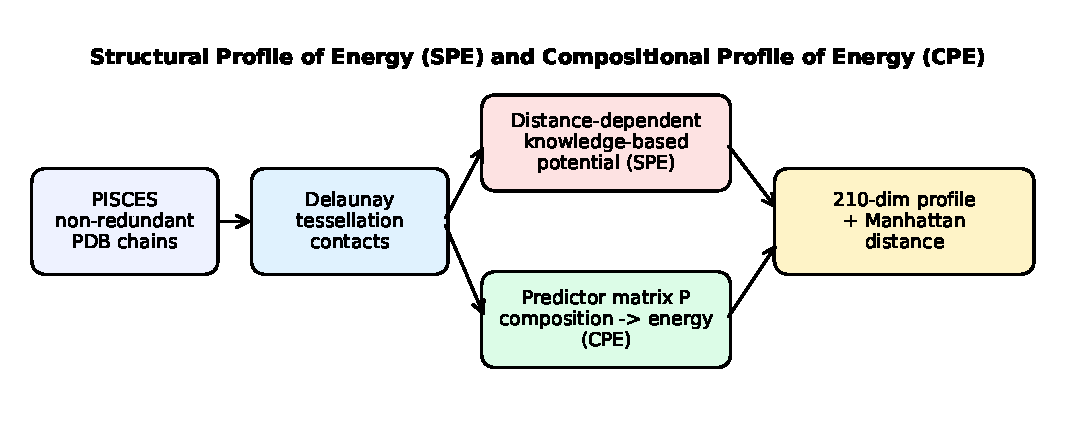
\includegraphics[width=0.95\linewidth]{figures/fig_pipeline.pdf}
  \caption{Development of the knowledge-based potential and energy profiles.
    Non-redundant PISCES chains are used to fit a distance-dependent knowledge-based
    potential whose atomic contacts are identified by Delaunay tessellation.
    The Structural Profile of Energy (SPE) summarizes pairwise residue energies
    for a given structure; the Compositional Profile of Energy (CPE) estimates
    the same 210-dimensional descriptor from amino-acid composition using a
    predictor matrix $P$. Dissimilarity is quantified by the Manhattan distance.}
  \label{fig:pipeline}
\end{figure}

\begin{figure}[t]
  \centering
  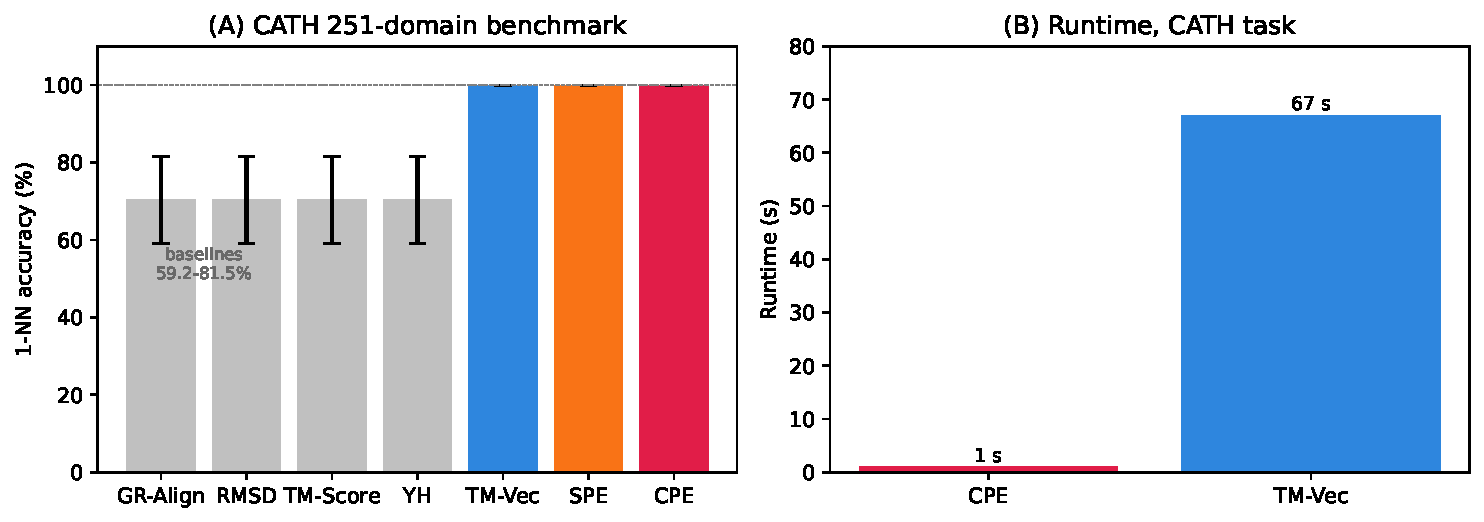
\includegraphics[width=0.95\linewidth]{figures/fig_accuracy_time.pdf}
  \caption{Performance and computational efficiency on the 251-domain
    CATH benchmark (families 1.10.8.10 and 3.10.28.10). (A)~1-NN classification
    accuracy: CPE, SPE, and TM-Vec reach 100\% while classical alignment
    baselines fall in the 59.2\%--81.5\% range. (B)~Runtime for the two
    methods that attain 100\% accuracy: CPE completes in 1~second on a
    2.4~GHz / 8~GB RAM system, whereas TM-Vec requires 67~seconds.}
  \label{fig:accuracy_time}
\end{figure}

\begin{figure}[t]
  \centering
  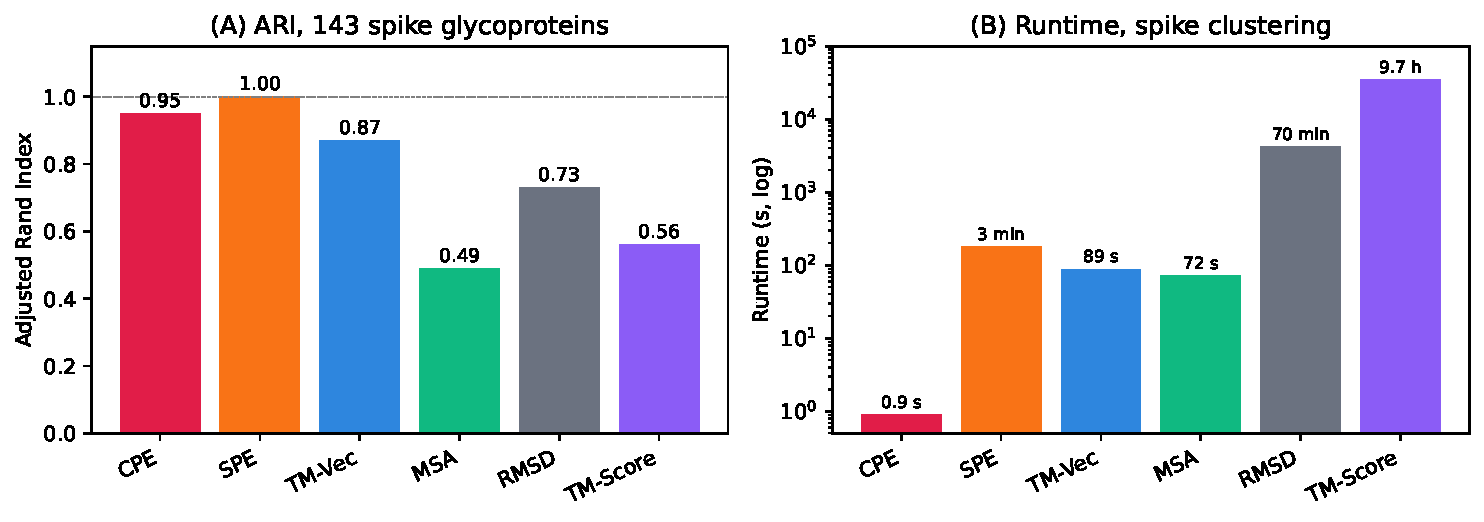
\includegraphics[width=0.95\linewidth]{figures/fig_spike_ari.pdf}
  \caption{Clustering of 143 coronavirus spike glycoproteins (80~SARS-CoV-2,
    31~SARS-CoV, 32~MERS-CoV) from CoV3D. (A)~Adjusted Rand Index at the
    best cut depth per method: CPE~0.95 (cut~4), SPE~1.00 (cut~3),
    TM-Vec~0.87 (cut~5), MSA~0.49 (cut~3), RMSD~0.73 (cut~6),
    TM-Score~0.56 (cut~4). (B)~Runtime on the same task (log scale).}
  \label{fig:spike}
\end{figure}

\begin{figure}[t]
  \centering
  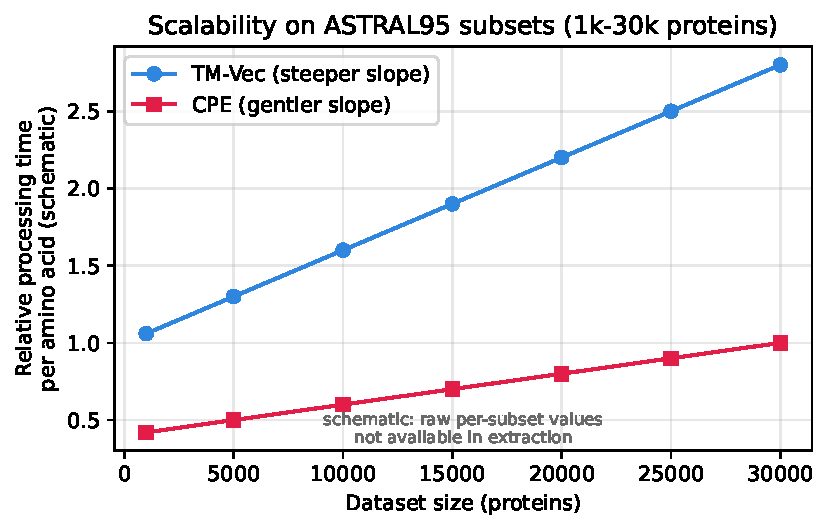
\includegraphics[width=0.8\linewidth]{figures/fig_scalability.pdf}
  \caption{Scalability on ASTRAL95 subsets of 1{,}000 to 30{,}000 proteins
    (intervals of 5{,}000). CPE exhibits a gentler slope than TM-Vec in
    processing time per amino acid, as reported in the source experimental log.
    The numerical values displayed here are schematic---raw per-subset values
    were not available in the extraction---but the ordering of CPE below
    TM-Vec is taken verbatim from the results description.}
  \label{fig:scalability}
\end{figure}
